\chapter{System Overview}

In order to understand the process of the recovery of rare earth elements from electronic waste with biosorption, the key procedures and techniques are described briefly in the following section.


\section{Detection and Measurement of REE concentration\authorA}

\subsection{Precipation Reactions}
A relatively simple proof if a probe contains REEs is a precipitation reaction.
The precipitation reactions a work because the rare earths form greater complexes with other molecules which have a different color than the surrounding solution ~\cite{janderblasius}.
As an example, a Ce precipitation reaction is shown in~\ref{fig:cer_precipitation_cropped} with an orange-red precipitate.

\begin{figure}[H]
    \centering
    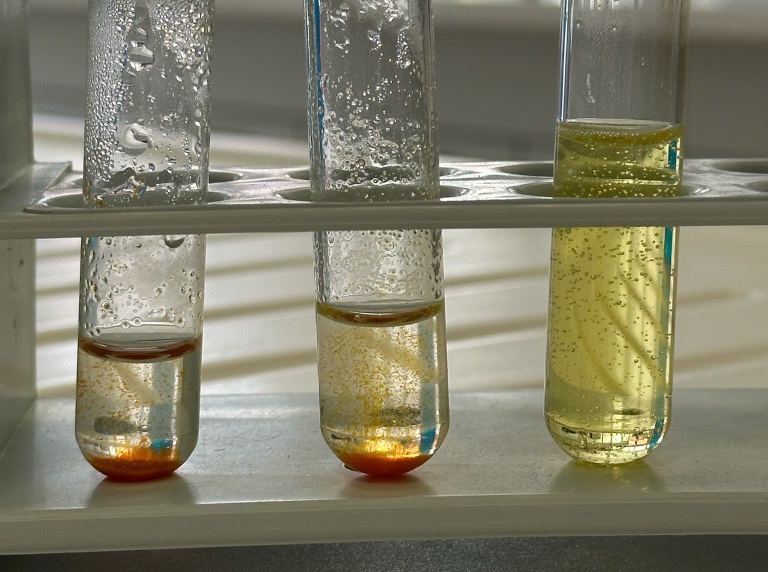
\includegraphics[width=0.8\textwidth]{./media/images/ree_precipitation_reaction_cropped}
    \caption{Precipitation of a successful REE detection reaction. The test tube on the righthandside does not show any precipitation because the probe was deionized water.}
    \label{fig:cer_precipitation_cropped}
\end{figure}

However, you must be careful because of the REEs chemical similarity, the detection of a specific REE is not always possible with these precipitation methods.
A precipitation reaction might also not be sensitive enough for your use case.
So it could be possible that your probe contains rare earths, but you were not able to detect them.

\subsection{Arsenazo III Assay}
A better and more versatile method to detect rare earths in a probe is the so-called arsenazo III assay.
With this assay, it is not only possible to detect if rare earths are present, but it is also possible to determine the concentration of REEs~\cite{arsenazo3assay}.

\begin{figure}[H]
    \centering
    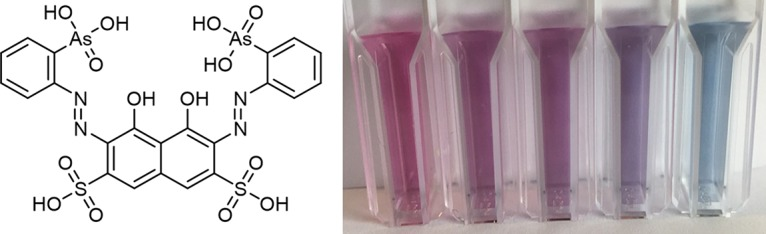
\includegraphics[width=0.9\textwidth]{media/images/arsenazo3_structure_example}
    \caption{Structure of arsenazo III. On the right you can see how the color of the dye changes with the levels of REE concentration. Picture from "Facile Arsenazo III-based assay for monitoring rare earth element depletion from cultivation media for methanotrophic and methylotrophic bacteria" Hoogendorn et al. \cite{arsenazo3assay}.}
    \label{fig:arsenazo3}
\end{figure}

Arsenazo III is a metallochromic dye.
This means that the dye changes its color depending on the presence of metal ions (for example:~\ref{fig:arsenazo3}).
A second crucial characteristic is that the color of an arsenazo III solution is also dependent on the concentration of some metal ions.
The metal ions and the arsenazo III molecule form complexes which block some certain frequencies of light.
This property can be used to determine the concentration of rare earths in a probe.

\newpage

\section{Methylorubrum extorquens}

\subsection{General information\authorB{}}

Utilizing a special strain of bacteria called \emph{Methylorubrum extorquens}, we can extract
these REEs from electronic waste. This works because the aforementioned bacteria
contains an amino acid called Lanmodulin which has the unique property of binding to
REEs. This technique allows us to wash REEs out of electronic waste in a similar way that
surfactants wash the dirt out of laundry.

\begin{figure}[H]
    \centering
    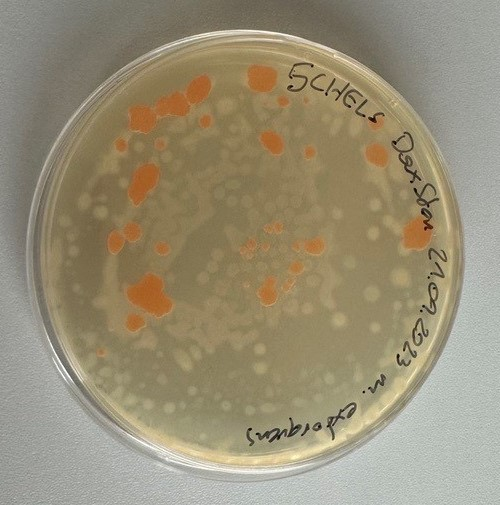
\includegraphics[width=0.6\textwidth]{./media/images/mextorquens_petri_dish}
    \caption{\emph{Methylorubrum extorquens} in a petri dish.}
    \label{fig:mextorquens_petri_dish}
\end{figure}

These bacteria reside in common soil, plant leaves, and dust and can also form symbiotic
relationships with said plants. The bacteria appear orange or pink when cultivated on a
solid or in a liquid medium. \emph{Methylorubrum extorquens} utilizes Methanol as an Energy
and Carbon source which is why we put Methanol in our nutrient medium.

\subsection{Lanmodulin\authorA}

Lanmodulin (LanM) is a protein produced by \textit{M. extorquens}, a lanthanide-utilizing bacteria~\cite{lanmdiscovery}.
LanM is not essential for the growth or survival of \textit{M. extorquens}, and it is only produced when the bacteria are in a medium with presence of \ce{Ln^{III}} or \ce{Ce^{III}} ions~\cite{lanmroleinbiology}.
However, the mechanisms that include LanM are not understood as a whole to this day.

\begin{figure}[H]
    \centering
    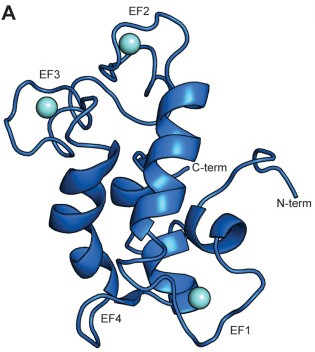
\includegraphics[width=0.6\textwidth]{./media/images/lanm_structure}
    \caption{Graphical visualization of Lanmodulins structure. EF indicates the EF hands, this is where the REEs can bind to the protein. In this visualization, the turquoise-colored spheres are \ce{Y^{III}} ions which are bound to the EF hands. Picture from "The biochemistry of lanthanide acquisition, trafficking and utilization", Emily R. Featherston and Joseph A. Cotruvo \cite{lanmroleinbiology}.}
    \label{fig:lanm_structure}
\end{figure}

The most important characteristic of LanM is that the molecule is able to bind lanthanide ions, primarily light REEs (LREEs).
When LanM does this, it undergoes a transformation from a disordered state to a compact form of itself.
The REEs are hereby bound to the so-called EF hands which favor to bind to \ce{Ln^{III}} and other lanthanoids over \ce{Ca^{II}} which is usually associated with these EF-hands~\cite{lanmstructure}.


\subsection{Protein Extraction/IR-Spectrometry\authorB{}}


\subsection{Cell Lysis\authorB{}}

\subsection{SDS-PAGE\authorB{}}
